% 编译: latexmk -xelatex paper_dpmzm_zh.tex
\documentclass[11pt,journal,onecolumn]{IEEEtran}
\usepackage{amsmath,amssymb,amsthm}
\usepackage{bm}
\usepackage{graphicx}
\usepackage{booktabs}
\usepackage{array}
\usepackage{cite}
\usepackage{algorithm}
\usepackage{algpseudocode}
\floatname{algorithm}{算法}
\renewcommand{\algorithmicrequire}{\textbf{输入:}}
\renewcommand{\algorithmicensure}{\textbf{输出:}}
\newcommand{\placeholderbox}[2]{\fbox{\parbox[c][#1][c]{0.9\linewidth}{\centering\textbf{【实测数据待补充】}\\[3pt]#2}}}
\usepackage{fontspec}
% Load by filename (kpathsea-searched in texmf-dist) for cross-platform builds
% (Windows/macOS/Linux) -- avoids OS font-name lookup and hardcoded paths.
\setmainfont{texgyretermes-regular.otf}[
  BoldFont=texgyretermes-bold.otf,
  ItalicFont=texgyretermes-italic.otf,
  BoldItalicFont=texgyretermes-bolditalic.otf]
\makeatletter
\edef\@tmp{\noexpand\DeclareFontFamilySubstitution{TU}{ptm}{\rmdefault}}\@tmp
\makeatother
\usepackage{xeCJK}
\setCJKmainfont[
  BoldFont={FandolSong-Bold.otf},
  ItalicFont={FandolKai-Regular.otf}
]{FandolSong-Regular.otf}
\setCJKsansfont[
  BoldFont={FandolHei-Bold.otf}
]{FandolHei-Regular.otf}
\setCJKmonofont{FandolFang-Regular.otf}
\usepackage{indentfirst}
\setlength{\parindent}{2em}
\usepackage[colorlinks=false,pdfborder={0 0 0}]{hyperref}

\renewcommand{\abstractname}{摘\quad 要}
\renewcommand{\IEEEkeywordsname}{关键词}
\renewcommand{\figurename}{图}
\renewcommand{\tablename}{表}
\renewcommand{\appendixname}{附录}
\renewcommand{\refname}{参考文献}

\theoremstyle{plain}
\newtheorem{theorem}{定理}
\newtheorem{lemma}{引理}
\newtheorem{proposition}{命题}
\theoremstyle{remark}
\newtheorem{remark}{注}
\renewcommand{\proofname}{证明}

\newcommand{\zv}{\mathbf{z}}
\newcommand{\uv}{\mathbf{u}}
\newcommand{\bv}{\mathbf{b}}
\newcommand{\nv}{\mathbf{n}}
\newcommand{\tv}{\mathbf{t}}
\newcommand{\vv}{\mathbf{v}}
\newcommand{\phiv}{\bm{\varphi}}
\newcommand{\Jc}{\mathcal{J}}
\newcommand{\Lc}{\mathcal{L}}
\newcommand{\atan}{\operatorname{atan2}}
\newcommand{\T}{\mathsf{T}}

\begin{document}

\title{DPMZM 三轴任意点偏压控制：$\mathbb{T}^3$ 上的仿射几何、IMD 可观测性与高斯--牛顿解调}

\author{第一作者，第二作者%
\thanks{论文草稿。作者姓名、单位与基金信息待补充。作者单位：西安电子科技大学综合业务网理论及关键技术国家重点实验室，西安~710071。}}

\markboth{预印本 --- DPMZM 三轴偏压控制的仿射框架}%
{作者~\MakeLowercase{\textit{等}}：DPMZM 任意点偏压控制的仿射几何}

\maketitle

\begin{abstract}
双平行马赫--曾德尔调制器（DPMZM）的三个偏置相位——两个子调制器与一个父干涉仪——通过输出强度耦合，标准 QPSK 点附近常用的解耦多环锁定依赖若干交叉项在该邻域内局部消失；一旦偏置需要停在传递曲面上的任意组合点（微波光子矢量调制、单边带权重控制），解耦假设不再成立，父偏置方向还会在标准点的一条轨道上变得不可观测。本文证明，在任意周期导频波形组和任意线性接收链下，DPMZM 的谐波解调观测向量是偏置状态三维环面~$\mathbb{T}^3$ 在一个含半角项的~12 维三角特征映射~$\Phi:\mathbb{T}^3\to\mathbb{R}^{12}$ 下的精确仿射像；该半角结构同时给出子轴~$4\pi$ 标定周期与~Klein 四元群构型等价的统一描述。观测雅可比的秩条件表明，六个谐波通道在标准~QPSK 工作点的~Klein 轨道上出现父轴不可观测，加入互调（IMD）通道~$\omega_1\pm\omega_2$ 等可在该点恢复满秩，但在~$\{c_1{=}c_2{=}0,\sin\varphi_3{=}0\}$ 处仍留有残余奇点。基于此，标定可由单条准周期扫描上的~$13\times13$ 线性回归完成，运行时解调采用热启动阻尼高斯--牛顿迭代，每控制周期计算量适合 Cortex-M 级控制器。数值验证显示：零噪声下辨识与解调闭合到数值精度；含噪声（$\sigma{=}0.002$）时解调偏差中位~$2.1$~mrad；在任意目标点与标准~QPSK 点，高斯--牛顿仿射控制器的闭环~rms 均保持~$17$--$19$~mrad，相对按传统解耦范式重构的三独立环基线（标准点~$358$--$397$~mrad rms，任意点~30 个失配实现中~23 个失锁）降低一至两个数量级。本文所报告的是理论推导与数值仿真结果；DPMZM 的台架实测尚待进行，实验章节给出已就绪的测量链路、分阶段计划与判据，作为下一步工作。该平台已在配套的单~MZM 论文~\cite{mzmaffine} 中完成实测验证，二者共用同一自研偏压控制硬件与仿射辨识—解调范式。
\end{abstract}

\begin{IEEEkeywords}
双平行~MZM，偏压控制，导频，仿射辨识，可观测性，高斯--牛顿，互调音，微波光子学。
\end{IEEEkeywords}

\IEEEpeerreviewmaketitle
\setlength{\emergencystretch}{2em}

\section*{符号说明}
\noindent\begin{tabular}{@{}>{$}l<{$}@{\quad}p{0.78\linewidth}@{}}
\xi(t),\,m & 导频时间波形与导频深度，$m=\pi V_d/V_\pi$\\
\eta & 消光系数，$\eta=2\sqrt r/(1+r)\le1$（$r$ 为臂间功率比）\\
\uv(\varphi_b) & 单~MZM 特征向量，$(\cos\varphi_b,\sin\varphi_b)^{\T}$\\
A,\bv,\nv & 仿射模型的矩阵、偏置与噪声\\
\kappa(A) & 观测矩阵~$A$ 的条件数（椭圆长短轴之比）\\
\mathbb{S}^1,\mathbb{T}^3 & 单~MZM 与~DPMZM 的偏置状态流形\\
\phiv & DPMZM 三偏置相位~$(\varphi_1,\varphi_2,\varphi_3)$（子~I、子~Q、父）\\
\Phi(\phiv) & DPMZM 的~12 维三角特征映射，$\Phi:\mathbb{T}^3\!\to\!\mathbb{R}^{12}$\\
J_n^{(i)},\,j_n^{(i)} & 全深度~$J_n(m_i)$ 与半深度~$J_n(m_i/2)$ Bessel 系数\\
c_i,s_i,C_3,S_3 & $\cos\frac{\varphi_i}{2},\sin\frac{\varphi_i}{2},\cos\varphi_3,\sin\varphi_3$\\
\Jc,\,\sigma_{\min} & 观测雅可比及其最小奇异值\\
V_4 & Klein 四元群（DPMZM 构型等价）\\
\end{tabular}

\section{引言}
\label{sec:intro}
双平行马赫--曾德尔调制器（DPMZM）把两个子马赫--曾德尔调制器（MZM）嵌套在一个父干涉仪中，是~IQ 矢量调制、单边带（SSB）产生和相干光发射机的核心器件~\cite{izutsu1981,yao2009,capmany2007}。三个偏置相位——子~I、子~Q、父——通过输出强度耦合；标准~QPSK 偏置点（双子零点、父正交）附近的解耦多环控制之所以可用，是因为在该邻域内若干交叉耦合项局部消失，三个环路可以近似独立锁定~\cite{cho2006,sotoodeh2011,kawakami2012,li2017}。

微波光子矢量调制、SSB 权重控制~\cite{izutsu1981}和模拟光计算~\cite{shen2017}等应用要求三轴偏置停在传递曲面上的一般组合点，而不只是标准~QPSK 点。此时解耦假设的两个支撑同时松动：离开标准点邻域后，交叉耦合项不再可忽略，三个"独立"环路实际上相互耦合；更根本的是，父偏置方向在标准点所在的一条轨道上直接不可观测——仅用子~I、子~Q、父三路自身的一、二次谐波，无法从观测中分离出父轴信息，与工作点是否在死区无关。已有的父轴可观测性修复借助非对称导频激发的互调（IMD）音~\cite{kawakami2012}，但该做法通常作为特殊点辅助手段引入，未被纳入一个覆盖整个~$\mathbb{T}^3$ 的统一辨识—解调框架。

配套论文~\cite{mzmaffine}证明，单~MZM 在任意周期导频和任意线性接收链下，谐波解调观测是偏置相位单位圆~$\mathbb{S}^1$ 的精确仿射像：偏置相位与导频波形在传递函数中因子化，线性非理想因素只改变仿射参数~$(A,\bv)$ 而不改变模型形式；据此可以把任意点控制写成"椭圆辨识、规范固定、$\atan$ 解调"的组合，其静态误差在配套论文的自研平台上得到了实测验证。本文的问题是，这一结构能否推广到状态空间从~$\mathbb{S}^1$ 变为~$\mathbb{T}^3$、观测曲面从二次簇变为一般三角簇的~DPMZM，以及父轴可观测性缺陷能否在同一框架内被系统地定位和修复。

本文证明，DPMZM 的半角耦合结构保持了观测对某个高维特征映射的仿射性，由此可以把三轴任意点控制同样归结为"辨识仿射参数、反演相位"的问题。本文的主要贡献如下：

\begin{enumerate}
\item \emph{DPMZM 的特征映射推广}。DPMZM 的半角结构把状态空间提升为~$\mathbb{T}^3$，并引出~12 维三角特征映射~$\Phi:\mathbb{T}^3\to\mathbb{R}^{12}$。对任意周期导频波形组、任意线性接收链与任意一组线性解调泛函，解调观测向量精确满足~$\zv=A\Phi(\phiv)+\bv+\nv$。该映射同时给出子轴~$4\pi$ 标定周期和~Klein 四元群构型等价的统一描述。
\item \emph{IMD 通道的可观测性解释}。六个谐波通道在标准~QPSK 点的~Klein 轨道上出现秩退化；加入互调通道~$\omega_1\!\pm\!\omega_2$~\cite{kawakami2012}后可在该点恢复父偏置方向的可观测性。本文同时指出九通道集在~$\{c_1{=}c_2{=}0,\ \sin\varphi_3{=}0\}$ 处仍有残余奇点。
\item \emph{面向实现的标定与解调算法}。DPMZM 标定可由单条准周期扫描上的线性回归完成，运行时解调采用热启动阻尼高斯--牛顿迭代。数值验证显示，该算法在给定仿真条件下达到毫弧度量级残差，计算量适合 Cortex-M 级控制器。
\item \emph{三轴闭环与解耦基线的定量对比}。给出统一覆盖标定、运行、残差监测与重定标的监督流程，并以按传统解耦多环范式重构的三独立环为基线，在任意目标点和标准~QPSK 点两种场景下量化仿射方法的闭环优势。
\end{enumerate}

在本文的仿真条件下，高斯--牛顿仿射控制器在任意目标点和标准~QPSK 点均把闭环~rms 稳定在~$17$--$19$~mrad，相对三独立环基线降低一至两个数量级，每控制周期计算量低于~$10^3$ 次乘加。DPMZM 的台架实测尚待进行；第~\ref{sec:exp} 节给出已就绪的测量链路、分阶段计划与判据。

第~\ref{sec:prelim} 节回顾单~MZM 仿射结果作为本文记号与结论的基础（细节见~\cite{mzmaffine}）；第~\ref{sec:dpmzm}--\ref{sec:gn} 节建立~DPMZM 的~$\mathbb{T}^3$ 几何、可观测性与标定解调理论；第~\ref{sec:algo} 节给出面向实现的标定与运行流程；第~\ref{sec:numerics} 节报告数值验证；第~\ref{sec:exp} 节给出实验验证方案；第~\ref{sec:discussion} 节讨论适用边界与~DP-QPSK 情形。

\section{预备：单~MZM 的精确仿射结果}
\label{sec:prelim}
本节压缩转述配套论文~\cite{mzmaffine}中与本文推导直接相关的记号与结论，细节和证明见该文。

\subsection{模型与仿射定理}
推挽式单驱~MZM 输出光功率
\begin{equation}
P_{\mathrm{out}}(t)=\tfrac{P_0}{2}\bigl[1+\eta\cos\varphi(t)\bigr],\quad
\eta=\tfrac{2\sqrt r}{1+r}\le 1,
\label{eq:mzm}
\end{equation}
其中~$\varphi(t)=\varphi_b+\xi(t)$，$\varphi_b=\pi V_b/V_\pi+\varphi_0$ 为偏置相位，标称导频~$\xi(t)=m\sin\omega t$，$m=\pi V_d/V_\pi$ 为导频深度。锁相解调取一次、二次谐波的线性泛函~$\Lc_1[f]\triangleq\overline{2f(t)\sin(\omega t{+}\theta_1)}$、$\Lc_2[f]\triangleq\overline{2f(t)\cos(2\omega t{+}\theta_2)}$，配以增益~$G_1,G_2$ 得观测~$Y\triangleq G_1\Lc_1[i]$、$X\triangleq G_2\Lc_2[i]$（下文~H1、H2 通道）。

关键结果是：对任意周期导频波形（不必正弦、不必小信号）与任意线性接收链，
\begin{equation}
\boxed{\;\zv=A\,\uv(\varphi_b)+\bv+\nv\;},\qquad
\uv(\varphi_b)=\begin{pmatrix}\cos\varphi_b\\\sin\varphi_b\end{pmatrix}
\label{eq:affine}
\end{equation}
精确成立——偏置相位与时间依赖的因子分解~$\cos(\varphi_b+\xi(t))=\cos\varphi_b\cos\xi(t)-\sin\varphi_b\sin\xi(t)$ 是其证明的核心。增益失配、参考相位误差、导频波形失真、相干串扰和有限消光比等线性非理想因素都进入仿射参数~$(A,\bv)$，模型形式不变；理想极限下~$A=\operatorname{diag}(\eta\kappa_2,-\eta\kappa_1)$，$\kappa_n\triangleq G_n\rho P_0 J_n(m)$ 为谐波斜率系数。

\subsection{标定、解调与噪声判据}
观测轨迹为椭圆~$(\zv-\bv)^{\T}M(\zv-\bv)=1$，$M=(AA^{\T})^{-1}\succ0$。椭圆有五个参数而~$(A,\bv)$ 有六个自由度，差额来自~$\mathbb{S}^1$ 的稳定子~$O(2)$；规范固定需要额外信息，单~MZM 情形下由直流通道提供相位原点、扫描方向提供定向。标定分四步：满周期慢扫记录观测；代数最小二乘拟合二次曲线得中心~$\hat\bv$ 与~$M$；由~$M^{1/2}$ 与轨道环绕方向得~$B_0$ 及反射~$F$；直流序列对~$(1,\cos\theta,\sin\theta)$ 的线性回归固定相位原点~$\hat\varphi_c$（相比~argmin 基准更稳健）。解调器为
\begin{equation}
B\triangleq R(-\hat\varphi_c)\,F\,M^{1/2},\qquad
\hat\varphi_b=\atan\!\bigl(B(\zv-\hat\bv)\bigr).
\label{eq:demod}
\end{equation}

噪声判据由观测矩阵的条件数给出：沿椭圆切向的一阶摄动给出相位方差~$\sigma^2_{\hat\varphi}\le\sigma^2/\sigma^2_{\min}(A)$，条件数~$\kappa(A)=\sqrt{\lambda_{\max}(M)/\lambda_{\min}(M)}$ 即椭圆长短轴之比；理想链路下~$\kappa(A)=J_1(m)/J_2(m)\to4/m$（小~$m$）。$\kappa(A)$ 因此是选择导频深度、评估观测质量的单一量化指标，本文~DPMZM 推广中将反复使用这一概念。配套论文~\cite{mzmaffine}在自研偏压控制平台上对单~MZM 实测验证了这一整套结构：任意点锁定相对~H1 幅值匹配基线误差降低约五倍（基线在死区完全失锁），并演示了残差触发的重定标闭环与小时级长期稳定；实测绝对精度由~$\kappa(A)$ 设定。本文使用与该平台相同的测量链路和控制范式，将其推广到~DPMZM 三轴场景。

\section{DPMZM：\texorpdfstring{$\mathbb{T}^3$}{T3} 上的几何}
\label{sec:dpmzm}

\subsection{场模型与半角结构}
DPMZM 由两个子~MZM 嵌套于父干涉仪构成，偏置相位~$\phiv=(\varphi_1,\varphi_2,\varphi_3)$。无~RF 数据时
\begin{align}
E_{\mathrm{out}}&=\frac{E_{\mathrm{in}}}{2}\Bigl[\cos\frac{\Theta_1}{2}
+e^{j\Theta_3}\cos\frac{\Theta_2}{2}\Bigr],\quad \Theta_i=\varphi_i+\xi_i(t),
\nonumber\\
P_{\mathrm{out}}&=\frac{P_0}{8}\bigl[2{+}\cos\Theta_1{+}\cos\Theta_2\bigr]
+\frac{P_0}{2}\cos\frac{\Theta_1}{2}\cos\frac{\Theta_2}{2}\cos\Theta_3.
\label{eq:dpmzm}
\end{align}
括号中的前两项对应两个子~MZM 的自项；最后一项来自父干涉仪的交叉干涉，并含有子相位的\emph{半角}。这一半角结构是 DPMZM 相对于单~MZM 的关键差异，并带来三个直接后果。

\emph{(i)~$4\pi$ 周期。}$\cos(\varphi_1/2)$ 的周期为~$4\pi$。当~$\varphi_1\!\to\!\varphi_1{+}2\pi$ 时，子~I 场和交叉项同时变号，输出强度可以区分这两个状态。因此，子轴标定扫描应覆盖~$4\pi$（电压~$4V_\pi$），即单~MZM 常规扫描范围的两倍。

\emph{(ii)~Klein 等价。}子场翻号配合父相位~$\pi$ 移相只改变场的全局符号：
\begin{equation*}
T_1:(\varphi_1{+}2\pi,\ \varphi_2,\ \varphi_3{+}\pi),\qquad
T_2:(\varphi_1,\ \varphi_2{+}2\pi,\ \varphi_3{+}\pi)
\end{equation*}
二者生成~$V_4=\{\mathrm{id},T_1,T_2,T_1T_2\}$；构型空间可写成商~$\widetilde{\mathbb{T}}^3/V_4$（图~\ref{fig:torus}）。对~QPSK 发射而言，该等价只对应星座重标记和全局相位变化。

\emph{(iii)}~标准~QPSK 偏置为~$(\pi,\pi,\pm\pi/2)$（双子零点、父正交、载波抑制）；任意点运行（微波光子矢量调制、SSB 权重）把三轴停驻在一般位置。

\begin{figure}[!htb]
\centering
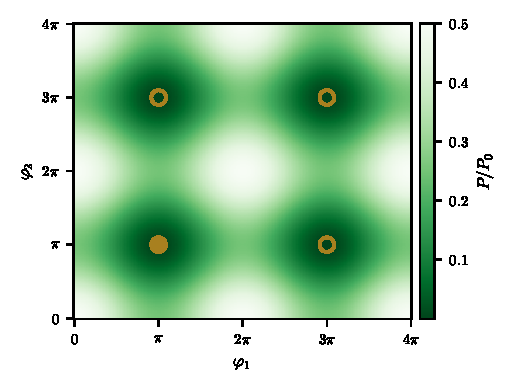
\includegraphics[width=0.55\textwidth]{figs/fig_torus.pdf}
\caption{DPMZM 强度~$P(\varphi_1,\varphi_2;\varphi_3{=}\pi/2)$，显示~$[0,4\pi)^2$ 区片。标准~QPSK 点（实心）与其三个~Klein 像（空心）具有相同强度，对应~$V_4$ 商结构。}
\label{fig:torus}
\end{figure}

\subsection{三音谐波观测与特征映射}
施加导频~$\xi_i=m_i\sin\omega_it$ 后，自项展开系数仍为全深度~Bessel 系数~$J_n^{(i)}\triangleq J_n(m_i)$，交叉项则按\emph{半深度}系数~$j_n^{(i)}\triangleq J_n(m_i/2)$ 展开。交叉项会产生互调谱线~$\omega_1{\pm}\omega_2$、$\omega_3{\pm}\omega_1$、$\omega_3{\pm}\omega_2$，这些谱线携带独立的相位信息，应作为观测通道处理。表~\ref{tab:dpchan} 列出本文采用的九通道首阶系数（$\rho P_0{=}1$、增益归一；$c_i{=}\cos\frac{\varphi_i}{2}$，$s_i{=}\sin\frac{\varphi_i}{2}$，$C_3{=}\cos\varphi_3$，$S_3{=}\sin\varphi_3$）。由这些系数可见，交叉耦合不宜视为小修正：在本文~$m_i{=}1.2$ 下，子轴交叉系数~$j_1^{(1)}j_0^{(2)}J_0(m_3)\approx0.18$ 约为自项斜率~$J_1(m_1)/4\approx0.12$ 的~$1.4$ 倍。实际频率规划还需保证~$\{\omega_i,2\omega_i,\omega_1{\pm}\omega_2,\omega_3{\pm}\omega_{1,2}\}$ 互不碰撞；本文仿真取~$\omega_{1,2,3}=1,1.37,1.93$。

\begin{table}[!t]
\caption{DPMZM 九通道的首阶系数}
\label{tab:dpchan}
\centering
\footnotesize
\setlength{\tabcolsep}{5pt}
\begin{tabular}{llll}
\toprule
通道 & 频率 & 首阶系数~$\times$ 单项式 & 角色\\
\midrule
$Y_1$ & $\omega_1$ & $-\frac14J_1^{(1)}\sin\varphi_1-j_1^{(1)}j_0^{(2)}J_0(m_3)\,s_1c_2C_3$ & 子~I 锁定\\
$X_1$ & $2\omega_1$ & $+\frac14J_2^{(1)}\cos\varphi_1+j_2^{(1)}j_0^{(2)}J_0(m_3)\,c_1c_2C_3$ & 判别\\
$Y_2$ & $\omega_2$ & $-\frac14J_1^{(2)}\sin\varphi_2-j_0^{(1)}j_1^{(2)}J_0(m_3)\,c_1s_2C_3$ & 子~Q 锁定\\
$X_2$ & $2\omega_2$ & $+\frac14J_2^{(2)}\cos\varphi_2+j_0^{(1)}j_2^{(2)}J_0(m_3)\,c_1c_2C_3$ & 判别\\
$Y_3$ & $\omega_3$ & $-j_0^{(1)}j_0^{(2)}J_1(m_3)\,c_1c_2S_3$ & 父（注意~$c_1c_2$）\\
$X_3$ & $2\omega_3$ & $+j_0^{(1)}j_0^{(2)}J_2(m_3)\,c_1c_2C_3$ & 父判别\\
$Z_-$ & $\omega_1{-}\omega_2$ & $+j_1^{(1)}j_1^{(2)}J_0(m_3)\,s_1s_2C_3$ & Kawakami 型~\cite{kawakami2012}\\
$Z_{13}$ & $\omega_3{-}\omega_1$ & $+j_1^{(1)}j_0^{(2)}J_1(m_3)\,s_1c_2S_3$ & 本文引入\\
$Z_{23}$ & $\omega_3{-}\omega_2$ & $+j_0^{(1)}j_1^{(2)}J_1(m_3)\,c_1s_2S_3$ & 本文引入\\
\bottomrule
\end{tabular}
\end{table}

对三个相位各应用一次相位因子分解（半角版本逐字成立），并三线性展开交叉项，光电流的~$\phiv$ 依赖只能由十二个三角单项式构成：
\begin{align}
\Phi(\phiv)&=\bigl(\underbrace{\cos\varphi_1,\sin\varphi_1,
\cos\varphi_2,\sin\varphi_2}_{\text{自项（全角）}},\;
\underbrace{\vv_1{\otimes}\vv_2{\otimes}\vv_3}_{\text{交叉项，8 维}}
\bigr),\nonumber\\
\vv_1&=(c_1,s_1),\quad \vv_2=(c_2,s_2),\quad \vv_3=(C_3,S_3).
\label{eq:feature}
\end{align}

\begin{theorem}[DPMZM 精确仿射性]
\label{th:dpmzm}
对任意周期导频波形组~$\{\xi_i\}$、任意线性接收链与任意一组~$K$ 个线性解调泛函，
\begin{equation}
\zv=A\,\Phi(\phiv)+\bv+\nv,\qquad A\in\mathbb{R}^{K\times 12}
\label{eq:dpaffine}
\end{equation}
精确成立。理想链路下~$A=A_0$ 由表~\ref{tab:dpchan} 给出，且高度稀疏（每行一至二个非零元，图~\ref{fig:ahat}）。
\end{theorem}

在单~MZM 中，非理想因素可以逐项写入~$A$ 和~$\bv$；在 DPMZM 中，更合适的做法是先固定特征映射~$\Phi$，再用线性回归辨识~$A$ 和~$\bv$，以吸收线性链路失配。规范自由度也相应推广：相位平移~$\varphi_i\to\varphi_i+\alpha_i$ 通过三角加法公式在特征空间中诱导线性作用，半角对按~$\alpha_i/2$ 旋转，全角对按~$\alpha_i$ 旋转，张量块按张量旋转。因此，$(A,\bv)$ 只能辨识到三个相位原点；这些原点逐轴由直流回归固定，反射由扫描方向固定，离散~$V_4$ 歧义由基本域约定处理。表~\ref{tab:struct} 总结两类器件的对应关系。

\begin{table}[!t]
\caption{结构对应：单~MZM 与~DPMZM}
\label{tab:struct}
\centering
\footnotesize
\setlength{\tabcolsep}{3pt}
\begin{tabular}{lll}
\toprule
要素 & 单~MZM & DPMZM\\
\midrule
状态流形 & $\mathbb{S}^1$ & $\mathbb{T}^3$（构型~$\widetilde{\mathbb{T}}^3/V_4$）\\
特征映射 & $\uv\in\mathbb{R}^2$（恒等） & $\Phi\in\mathbb{R}^{12}$（含半角）\\
轴向周期 & $2\pi$ & 子轴~$4\pi$，父轴~$2\pi$\\
通道数 & 2（$\omega,2\omega$） & $\ge 7$，IMD 必需\\
曲面拟合 & 椭圆（二次簇） & 准周期扫描回归\\
规范群 & $O(2)$ & $\mathbb{T}^3\rtimes(\text{反射}\times V_4)$\\
解调 & $\atan$（闭式） & 热启动高斯--牛顿\\
不可观修复 & H1/H2 联用 & IMD 通道\\
\bottomrule
\end{tabular}
\end{table}

\section{可观测性与~IMD 通道的必要性}
\label{sec:obs}
解调的局部可行性由观测雅可比~$\Jc(\phiv)=A\,D\Phi(\phiv)\in\mathbb{R}^{K\times3}$ 的秩条件~$\sigma_{\min}(\Jc)>0$ 刻画，这是单~MZM 情形下浸入论证~\cite{mzmaffine}的三维推广。与圆嵌入不同，DPMZM 的被观测嵌入可能在某些偏置组合处退化；标准~QPSK 点正是需要重点检查的位置。

\begin{proposition}[标准点不可观及其奇异轨迹]
\label{prop:blind}
取表~\ref{tab:dpchan} 中六个谐波通道~$Y_{1,2,3},X_{1,2,3}$ 与理想~$A_0$。使~$\partial\zv/\partial\varphi_3=\mathbf{0}$（父轴不可观）的集合为~$\{c_1=c_2=0\}$，即\emph{标准~QPSK 工作点的~Klein 轨道}，且对任意~$\varphi_3$ 成立。加入~IMD 通道~$Z_-$ 后，单项式~$s_1s_2C_3$ 的~$\varphi_3$ 偏导在标准点为~$-s_1s_2S_3=\mp1$，从而在该处恢复满秩。
\end{proposition}
\begin{proof}[证明梗概]
六通道所含交叉单项式的~$\varphi_3$ 偏导（略去正的深度系数）分别为~$-s_1c_2S_3$（$Y_1$）、$-c_1s_2S_3$（$Y_2$）、$-c_1c_2S_3$（$X_1,X_2,X_3$）与~$+c_1c_2C_3$（$Y_3$）。若这些项对任意~$\varphi_3$ 同时为零，则需要~$s_1c_2=c_1s_2=c_1c_2=0$，其解为~$c_1=c_2=0$；另一支~$s_1=s_2=0$ 与~$c_1c_2=0$ 矛盾。数值上，标准点处六通道~$\sigma_{\min}$ 降至机器精度（数值上为零，实测~$\sim10^{-33}$），加入~$Z_-$ 后恢复为~$5.5\times10^{-2}$。
\end{proof}

因此，六个谐波通道在标准~QPSK 点附近缺少父偏置方向的信息。文献中使用~IMD 音检测父偏置~\cite{kawakami2012}，在这里可解释为恢复雅可比秩的需要。仍需注意一处残余奇点：在~$\{c_1{=}c_2{=}0,\ S_3{=}0\}$（如~$(\pi,\pi,0)$，输出全暗）处，父相位信息落在未观测的单项式~$s_1s_2S_3$ 上，九通道下仍有~$\sigma_{\min}=1.1\times10^{-17}$；可通过三阶~IMD~$\omega_1{+}\omega_2{\pm}\omega_3$ 或路径绕行处理。图~\ref{fig:obs} 给出~$[0,4\pi)^2$ 上的~$\log_{10}\sigma_{\min}(\Jc)$：六通道低秩区域落在~Klein 轨道上，九通道在~$\varphi_3=\pi/2$ 处恢复可观测性，而~$\varphi_3=0$ 切片上出现上述残余奇点。

\begin{figure}[!htb]
\centering
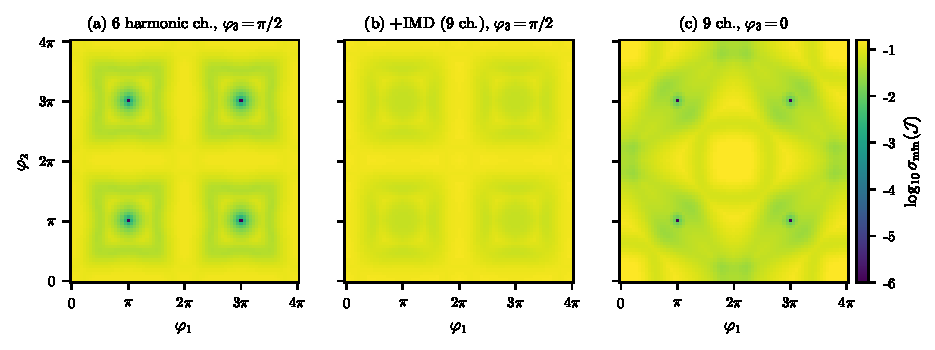
\includegraphics[width=0.92\textwidth]{figs/fig_obs.pdf}
\caption{可观测性热图~$\log_{10}\sigma_{\min}(\Jc)$，$(\varphi_1,\varphi_2)\in[0,4\pi)^2$。(a)~六谐波通道、$\varphi_3{=}\pi/2$：低秩区域位于标准~QPSK 点的~Klein 轨道上。(b)~加入三个~IMD 通道后可观测性恢复。(c)~九通道、$\varphi_3{=}0$：命题~\ref{prop:blind} 的残余奇点在同一轨道上出现。}
\label{fig:obs}
\end{figure}

\section{\texorpdfstring{$\mathbb{T}^3$}{T3} 上的标定与高斯--牛顿解调}
\label{sec:gn}
单~MZM 的标定可以利用观测椭圆的二次曲线结构~\cite{mzmaffine}。DPMZM 中的~$\Phi(\mathbb{T}^3)$ 不再是二次簇，因而没有对应的闭式椭圆拟合；但定理~\ref{th:dpmzm} 给出另一条路：观测对特征~$\Phi$ 仍为线性，故在规范固定坐标下可用普通最小二乘辨识
\begin{equation}
[\hat A\,|\,\hat\bv]
=\Bigl(\sum_k\zv_k\tilde\Phi_k^{\T}\Bigr)
\Bigl(\sum_k\tilde\Phi_k\tilde\Phi_k^{\T}\Bigr)^{-1},\quad
\tilde\Phi=\begin{pmatrix}\Phi\\1\end{pmatrix},
\label{eq:regress}
\end{equation}
一次~$13{\times}13$ Gram 分解可服务所有~$K$ 个通道。无需三维网格扫描；取增量比无理的\emph{准周期}轨线~$\varphi_i(k)=k\Delta_i$（此处~$\Delta=(0.0424,0.0532,0.0679)$），单条轨线可覆盖~$\mathbb{T}^3$ 的不同区域，$N=3000$ 个样本得到良态~Gram 矩阵。各轴标度~$V_{\pi,i}$ 由扫描数据的基波周期估计获得（子轴周期~$4\pi$），相位原点由逐轴直流回归固定。

运行时解调则从闭式~$\atan$ 推广为迭代求解（图~\ref{fig:arch}）。圆嵌入有全局闭式逆，$\Phi(\mathbb{T}^3)$ 没有；但偏压控制是跟踪问题，可用上一周期估计作为热启动，执行阻尼高斯--牛顿步~\cite{nocedal2006}
\begin{equation}
\hat\phiv\leftarrow\hat\phiv+(\Jc^{\T}\Jc+\lambda I)^{-1}
\Jc^{\T}\bigl[\zv-\hat A\Phi(\hat\phiv)-\hat\bv\bigr],
\label{eq:gn}
\end{equation}
在本文仿真设置下，两次迭代可达到测量噪声地板。收敛域由~$\sigma_{\min}(\Jc)$ 与嵌入曲率共同决定，因此图~\ref{fig:obs} 也可作为解调条件数的参考图。借助~$\hat A$ 的稀疏性，每控制周期需要约数百次乘加和一次~$3{\times}3$ 求解；相对于锁相处理本身，该开销适合 Cortex-M 级控制器。解调后误差~$\mathbf{e}=\hat\phiv-\phiv^\ast$ 可按三轴相位误差进入控制律。

\begin{figure}[!htb]
\centering
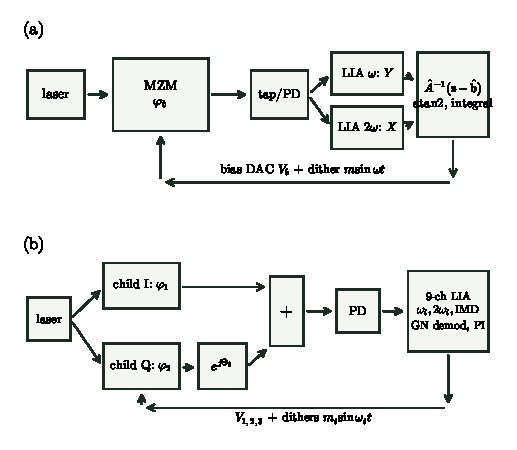
\includegraphics[width=0.62\textwidth]{figs/fig_arch.pdf}
\caption{DPMZM 控制架构：九路锁相通道（谐波与互调音）馈入本节的高斯--牛顿解调器，输出三轴相位误差写回~PI 更新。}
\label{fig:arch}
\end{figure}

\emph{噪声地板与导频深度设计。}估计协方差为~Cram\'er--Rao 型~$\Sigma_{\hat\phiv}=(\Jc^{\T}\Sigma_n^{-1}\Jc)^{-1}$，其~$K{=}2$ 时的插入式对应即单~MZM 情形下的~$\sigma^2_{\hat\varphi}\le\sigma^2/\sigma^2_{\min}(A)$。与单~MZM 不同，条件数此时由二阶小的~IMD 系数主导：双子零点附近父相位方差
\begin{equation}
\sigma^2_{\hat\varphi_3}\approx
\frac{\sigma^2}{\bigl[j_1^{(1)}j_1^{(2)}J_0(m_3)\bigr]^2}
\approx\Bigl(\frac{16}{m_1m_2}\Bigr)^{2}\sigma^2,
\label{eq:parentnoise}
\end{equation}
高于子轴地板~$(8/m)^2\sigma^2$：二者之比~$\propto1/m^2$，在本文~$m{=}1.2$ 下约~$3$--$5$ 倍，随导频深度变浅迅速增大，浅导频（如配套论文实测台~$m\approx0.13$~\cite{mzmaffine}）时可达一个量级以上；其对~$1/m$ 的依赖也由一次方升为二次方。因此，DPMZM 的导频深度需要优先满足父轴~IMD 信噪比，而不能直接沿用单~MZM 的经验取值。

对照基线并非取自某一篇文献，而是按传统解耦多环范式~\cite{cho2006,sotoodeh2011,kawakami2012,li2017} 重构的代表性方案：三个独立单环分别锁定子~I、子~Q 与父偏置，其中父偏置沿用~Kawakami 的非对称导频~IMD 音检测~\cite{kawakami2012}。具体地，误差量取~$(Y_1,Y_2,Z_-)$，参考值由理想模型~$A_0\Phi(\phiv^\ast)$ 计算，斜率取理想雅可比的\emph{对角元}。与本文方法的区别在于：该基线保留了理想耦合项，但既不进行矩阵反演，也不辨识~$A\neq A_0$ 和~$\bv\neq0$ 的线性失配。在标准点附近，部分交叉项局部消失，解耦设计可以成立；但静差会经二阶小的父轴斜率~$j_1^{(1)}j_1^{(2)}J_0(m_3)$ 放大。对于任意目标点，还会叠加跨轴耦合与死区效应。

\begin{figure}[!htb]
\centering
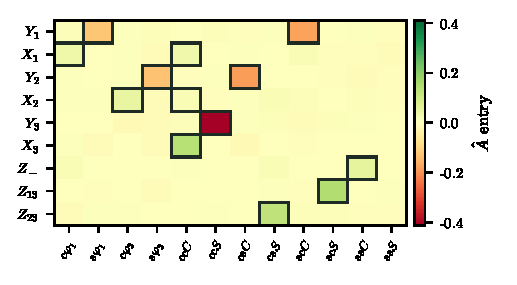
\includegraphics[width=0.6\textwidth]{figs/fig_ahat.pdf}
\caption{DPMZM 线性回归辨识：回归所得~$\hat A$（色块）对照理想~$A_0$ 的稀疏指纹（方框）。指纹外的元素来自注入的非结构化扰动~$\delta_A{=}0.12$，回归能够估计这些线性失配。}
\label{fig:ahat}
\end{figure}

\section{基于仿射模型的偏压控制算法设计}
\label{sec:algo}
前述理论可组织成一个两阶段控制流程（图~\ref{fig:flow}）。标定阶段执行偏压扫描、模型拟合、规范固定和残差自检；运行阶段在每个控制周期读取锁相输出，完成相位解调、误差计算和 PI 更新，并用模型残差监测链路是否偏离标定状态。若残差持续越限，则触发微幅弧重定标。算法~\ref{alg:cal} 与算法~\ref{alg:run} 给出两阶段伪代码，统一覆盖标定/回归拟合与~$\atan$/高斯--牛顿解调两条支路——单~MZM 支路对应配套论文~\cite{mzmaffine}的流程，DPMZM 支路是本文的推广对象。

\begin{figure}[!htb]
\centering
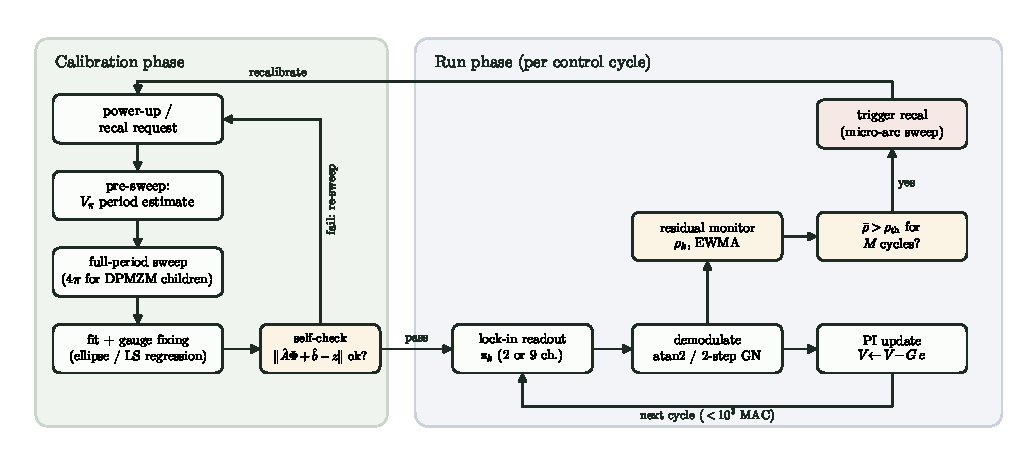
\includegraphics[width=0.95\textwidth]{figs/fig_flow.pdf}
\caption{监督状态机：左为标定阶段（扫描$\to$拟合与规范固定$\to$自检），右为运行阶段的每周期回路（锁相读出$\to$解调$\to$PI$\to$残差监测），残差越限持续~$M$ 周期即触发微幅弧重定标并返回标定通道。}
\label{fig:flow}
\end{figure}

\begin{algorithm}[!t]
\caption{自标定与规范固定（上电或重定标触发时执行）}
\label{alg:cal}
\begin{algorithmic}[1]
\Require 样本数~$N$；通道集~$K{=}9$（含~IMD）
\Ensure 解调参数~$\hat A,\hat\bv$ 与残差阈值~$\rho_{\rm th}$
\State 预扫描估计各轴~$V_{\pi,i}$（基波周期；子轴按~$4\pi$ 周期）
\State 取准周期轨线~$\varphi_i(k)=k\Delta_i$（增量比无理）记录~$\{\zv_k,\bar\imath_k\}_{k=1}^N$
\State 构造~$\tilde\Phi_k=(\Phi(\phiv_k)^{\T},1)^{\T}$；解~$13{\times}13$ 法方程得~$[\hat A\,|\,\hat\bv]$（式~\eqref{eq:regress}）
\State 逐轴直流回归固定三个相位原点；按基本域约定消解~$V_4$ 歧义
\State 自检：$\max_k\|\zv_k-\hat A\Phi_k-\hat\bv\|<\epsilon_{\rm cal}$？不通过则重新扫描
\State 记录残差统计~$(\mu_\rho,\sigma_\rho)$，置~$\rho_{\rm th}=\mu_\rho+k_\sigma\sigma_\rho$（$k_\sigma\approx4$--$6$）
\end{algorithmic}
\end{algorithm}

\begin{algorithm}[!t]
\caption{运行时控制周期（含残差监测与重定标触发）}
\label{alg:run}
\begin{algorithmic}[1]
\Require 目标~$\phiv^\ast$、环路增益~$G$、阈值对~$(\rho_{\rm th},M)$、上周期估计~$\hat\phiv^-$
\State 读取锁相输出~$\zv_k$
\State 以~$\hat\phiv^-$ 热启动执行两步阻尼高斯--牛顿（式~\eqref{eq:gn}）得~$\hat\phiv$；$\rho_k\gets\|\zv_k-\hat A\Phi(\hat\phiv)-\hat\bv\|$
\State $\mathbf e\gets\operatorname{wrap}(\hat\phiv-\phiv^\ast)$；\quad PI 更新~$V\gets V-G\,\mathbf e\cdot V_\pi/\pi$ 写入偏压~DAC
\State 残差~EWMA：$\bar\rho\gets(1-\lambda)\bar\rho+\lambda\rho_k$
\If{$\bar\rho>\rho_{\rm th}$ 连续~$M$ 周期}
  \State 保持当前~$V$，执行微幅弧重定标（调用算法~\ref{alg:cal}；弧优先激励~$s_1s_2$ 子空间）
\EndIf
\Ensure 进入下一周期；全周期代价~$<10^3$ 次乘加
\end{algorithmic}
\end{algorithm}

实现时有三类参数需要整定。\emph{阈值整定}：$\rho_{\rm th}$ 由标定末尾的残差分布给出，配合~EWMA（$\lambda\approx0.05$）和连续~$M$ 周期判决（$M\approx20$--$30$），可在误触发率和检测延迟之间折中；延迟量级约为~$M+1/\lambda$ 个控制周期。\emph{重定标弧}：本文仿真采用~$\pm0.3$~rad 量级的微幅弧，以重新激励局部可辨识子空间，尤其是~IMD 相关、系数较弱的~$s_1s_2$ 方向；期间偏压保持在上一控制值附近，附加扰动与常规导频包络同量级。\emph{定点化}：高斯--牛顿中的~$3{\times}3$ 求解可用~Cholesky 分解展开为定长乘加序列。参数存储量为~$9{\times}12{+}9=117$ 个标量。

\section{数值验证}
\label{sec:numerics}

\subsection{仿真设置与主要结果}
数值验证使用受扰真值~$A_{\mathrm{true}}=A_0+\delta_A\,\Delta A$、$\bv_{\mathrm{true}}=\delta_b\,\Delta\bv$ 生成数据，其中~$\Delta A,\Delta\bv$ 为固定伪随机扰动，$\delta_A{=}0.12$ 表示相对~Frobenius 尺度，$\delta_b$ 对应~${\sim}10^{-2}$ 量级偏置。仿真同时叠加逐通道高斯噪声和共同漂移序列（随机游走加慢正弦），并对比较中的控制器施加同源漂移。DPMZM 参数为~$m_i{=}1.2$、$\sigma{=}0.002$、$N{=}3000$。主要结果汇总于表~\ref{tab:results}。

\begin{table}[!t]
\caption{数值验证汇总（DPMZM）}
\label{tab:results}
\centering
\footnotesize
\setlength{\tabcolsep}{5pt}
\begin{tabular}{ll}
\toprule
量 & 结果\\
\midrule
$D\Phi$ 对有限差分 & 最大~$7.7\times10^{-10}$\\
Klein 不变性~$\|\Phi\circ T_1-\Phi\|$ & $2.5\times10^{-15}$\\
零噪声辨识 / GN 恢复 & $<10^{-12}\%$ / $<10^{-12}$~mrad\\
含噪辨识（$\sigma{=}0.002$）/ 解调偏差 & $0.17\%$ / 中位~$2.1$、P95~$4.3$~mrad\\
$\sigma_{\min}$：六通道 / 九通道（标准点） & $\approx 0$（机器精度）/ $5.5\times10^{-2}$\\
$\sigma_{\min}$：九通道于~$(\pi,\pi,0)$ & $1.1\times10^{-17}$\\
闭环（任意目标点） & GN~$17.2$ / 三环~$358$~mrad（rms）\\
闭环（标准目标点） & GN~$18.5$ / 三环~$397$~mrad（rms）\\
三环静差，30 个失配实现 & 标准点：中位~$292$~[184,393]~mrad\\
 & 任意点：$23/30$ 失锁；余者中位~$417$~mrad\\
\midrule
\multicolumn{2}{l}{\emph{算法级动态（第~\ref{sec:algo} 节算法）}}\\
捕获时间常数（理论~$1/G$） & $6.2$ 周期\\
阶跃整定（至~$20$~mrad） & 与目标点无关，同量级于单~MZM 结果~\cite{mzmaffine}\\
\bottomrule
\end{tabular}
\end{table}

零噪声实验首先检验模型闭合性：线性回归辨识与高斯--牛顿解调（自~$0.3$~rad 热启动偏差恢复）均闭合到数值精度（辨识误差~$<10^{-12}\%$，恢复误差~$<10^{-12}$~mrad）。这一结果说明，式~\eqref{eq:dpaffine} 在仿真模型内为精确结构，而非小信号近似。

含噪辨识考察规范固定和模型反演的稳定性：在~$\sigma{=}0.002$ 时，辨识相对误差为~$0.17\%$，解调偏差中位为~$2.1$~mrad、P95 为~$4.3$~mrad。

闭环对比给出本文的核心结果。三环基线在任意目标点和标准目标点均可收敛，但分别留下~$358$ 和~$397$~mrad rms 误差；高斯--牛顿仿射控制器在两处保持~$17.2$ 和~$18.5$~mrad rms（图~\ref{fig:dploop}）。30 个失配实现的蒙特卡洛结果进一步显示，三环基线在标准点的静差中位为~$292$~mrad（IQR~$184$--$393$），在任意目标点有~$23/30$ 个实现失锁；高斯--牛顿仿射控制器保持在~$16$--$19$~mrad rms 范围内（图~\ref{fig:mcdp}）。

可观测性热图（图~\ref{fig:obs}）与命题~\ref{prop:blind} 一致：六谐波通道在标准~QPSK 点的~Klein 轨道附近出现低秩区域，加入~IMD 通道后在~$\varphi_3=\pi/2$ 切片恢复可观测性；当~$S_3=0$ 时，九通道残余奇点仍按理论预期出现。

\begin{figure}[!htb]
\centering
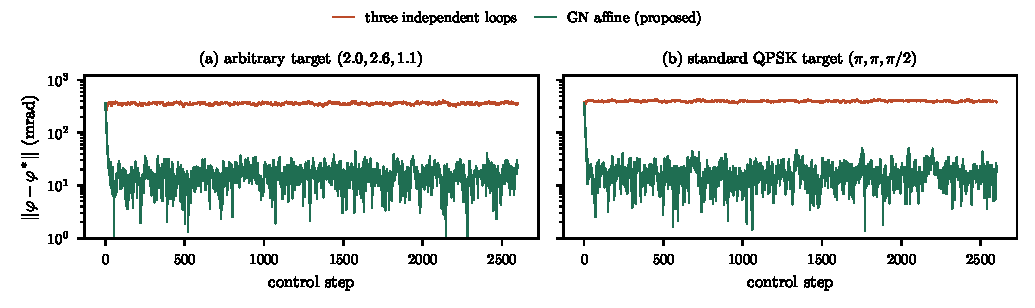
\includegraphics[width=0.85\textwidth]{figs/fig_dploop.pdf}
\caption{DPMZM 闭环跟踪，同源漂移，$\sigma{=}0.002$、$\delta_A{=}0.12$（对数误差轴）。(a)~任意目标点：三环基线携带~${\sim}0.36$~rad 静差；(b)~即使在标准~QPSK 点，基线仍经二阶小的父轴斜率继承可比静差，而高斯--牛顿仿射控制器在两处均保持~${\sim}18$~mrad（rms）。}
\label{fig:dploop}
\end{figure}

\begin{figure}[!htb]
\centering
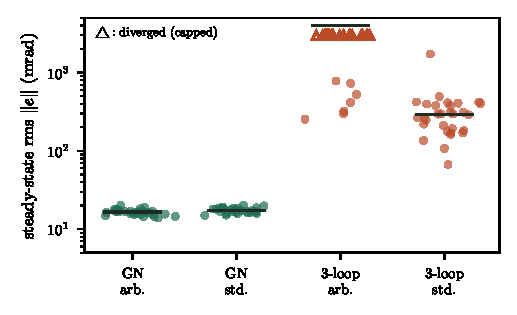
\includegraphics[width=0.58\textwidth]{figs/fig_mcdp.pdf}
\caption{DPMZM 静差的蒙特卡洛分布（30 个失配实现，横杠为中位数）：高斯--牛顿仿射控制器在任意与标准目标处均停留在测量噪声地板；三环基线携带数百毫弧度静差，且在任意目标处出现发散实现（三角标记，截幅显示）。}
\label{fig:mcdp}
\end{figure}

\subsection{算法级行为验证}
捕获瞬态从~$\|\Delta\phiv\|\approx0.96$~rad 的初始偏差出发，不同目标点的误差衰减曲线基本重合，并与理论包络~$(1-G)^n$ 一致，对应时间常数~$1/G\approx6.2$ 个周期，与配套论文~\cite{mzmaffine}中单~MZM 的~$5.6$ 周期同量级（两者环路增益~$G$ 取值不同）。三轴联合阶跃同样表现出目标点无关的整定动态，整定时间与单~MZM 结果~\cite{mzmaffine}处于同一量级。这些行为与算法~\ref{alg:cal}--\ref{alg:run} 中"标定—运行—残差监测—重定标"的统一骨架一致；残差触发重定标的具体时序（检测延迟、恢复精度）已在单~MZM 平台上实测验证~\cite{mzmaffine}，DPMZM 的对应实测见第~\ref{sec:exp} 节的计划阶段。

\section{实验验证}
\label{sec:exp}
本节给出~DPMZM 三轴任意点控制的实验验证方案：测量链路已经就绪，具体的三轴锁定实测尚待进行。自研偏压控制平台已在配套论文~\cite{mzmaffine}中完成单~MZM 的实测验证（任意点锁定 rms 约为~H1 幅值匹配基线的五分之一，基线在死区完全失锁，并演示了残差触发的重定标闭环与小时级长期稳定）；本节说明该平台扩展到~DPMZM 三轴场景所需的链路、分阶段计划与判据。

\emph{测量链路。}计划链路见图~\ref{fig:exp_dpmzm}，与单~MZM 链路~\cite{mzmaffine}同构：分布反馈激光器入射被测~DPMZM，输出经耦合器分出小比例至光电探测器（PD），PD 电流经跨阻放大后由自研~STM32H523 偏压控制板采集。区别在于三路子/父偏置与三音导频（$\omega_1,\omega_2,\omega_3$）：本板~DAC8568 提供八路偏置输出，覆盖三个偏置轴（含子轴~$4V_\pi$ 扫描范围）绰绰有余；板上~\texttt{gen} 命令支持最多三音导频，\texttt{acq} 命令可同时读取六个谐波通道与三个互调（IMD）通道，对应表~\ref{tab:dpchan} 的九通道观测。仿射标定（式~\eqref{eq:regress}）与高斯--牛顿反演（式~\eqref{eq:gn}）仍在上位机执行，板卡承担"导频/偏置发生器~$+$~谐波采集器"角色，与单~MZM 实验中的分工一致~\cite{mzmaffine}。

\begin{figure}[!htb]
\centering
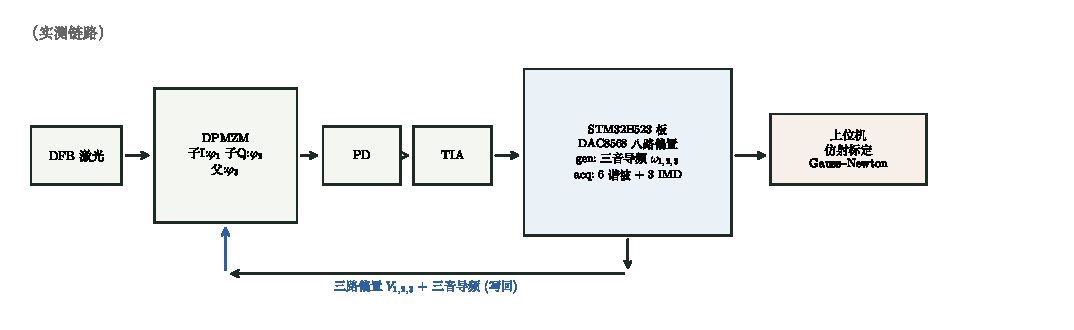
\includegraphics[width=0.95\textwidth]{figs/fig_exp_dpmzm.pdf}
\caption{DPMZM 待实测扩展链路（计划）。三路子/父偏置与三音导频（$\omega_1,\omega_2,\omega_3$）由~DAC8568 的八路偏置与~\texttt{gen} 多音能力（$\le3$ 导频）承担，板上~\texttt{acq} 同时读取六谐波与三个互调（IMD）通道；仿射标定与~Gauss--Newton 反演在上位机执行。}
\label{fig:exp_dpmzm}
\end{figure}

\emph{相位真值与精度评定。}沿用单~MZM 实验中的开环慢扫描评定法~\cite{mzmaffine}：用台式万用表记录整条直流传递曲线，由相邻极值定出~$V_\pi$ 与相位原点，作为锁定误差的独立基准。DPMZM 需在固定父偏置下逐子轴重复该扫描，子轴按~$4\pi$ 周期扫描以确认~$4\pi$ 标定周期本身（计划阶段（1））。

\emph{分阶段流程与判据。}DPMZM 实测按以下阶段推进，每阶段对照本文一张仿真图：
（1）子轴~$4\pi$ 与~Klein 等价——子~MZM 扫~$4V_\pi$，验证~$\varphi$ 与~$\varphi{+}2\pi$ 在输出上可区分（图~\ref{fig:exp6}~$\leftrightarrow$~图~\ref{fig:torus}）；
（2）可观测性恢复——标准~QPSK 点附近测父轴环路增益与解调方差，对比六谐波通道与加入~IMD 后的九通道（图~\ref{fig:exp5}~$\leftrightarrow$~图~\ref{fig:obs}）；
（3）任意点三轴锁定——对比三独立环的失锁率与静差（图~\ref{fig:exp4}~$\leftrightarrow$~图~\ref{fig:dploop}）。
判据：（1）子轴~$4\pi$ 扫描应观测到~$\varphi$ 与~$\varphi{+}2\pi$ 输出可区分，与~$2\pi$ 周期假设下的预测形成对照；（2）IMD 通道确能在标准点附近恢复父偏置可观测性，即九通道下父轴环路增益/解调方差应显著优于六通道；（3）任意点三轴~rms 显著优于三独立环基线，且不随目标点系统性放大。受交流通道余量限制，各项绝对指标预期高于本文~$m_i{=}1.2$ 仿真，参照单~MZM 实测中~$\kappa(A)$ 主导绝对精度的结论~\cite{mzmaffine}，DPMZM 实测的量级对比也应以趋势与相对优势为准，而非绝对数值。

\begin{table}[!t]
\caption{DPMZM 实验测试矩阵（计划）。仿真对照值来自表~\ref{tab:results}。}
\label{tab:exp}
\centering
\footnotesize
\setlength{\tabcolsep}{6pt}
\begin{tabular}{lll}
\toprule
指标 & 仿真值 & 实验值\\
\midrule
子轴~$4\pi$ 周期确认 & 定性可区分 & 计划\\
准周期扫描辨识~relF & $0.17\%$ & 计划\\
IMD 可观测性~$\sigma_{\min}$（六~$\to$ 九通道，标准点） & $\approx 0\to 5.5\times10^{-2}$ & 计划\\
任意点三轴~rms（GN / 三环） & $17.2$ / $358$~mrad & 计划\\
标准点三轴~rms（GN / 三环） & $18.5$ / $397$~mrad & 计划\\
\bottomrule
\end{tabular}
\par\footnotesize 注：仿真列取~$m_i{=}1.2$；实验列受交流通道余量限制，预期可用导频深度显著小于仿真值（参照单~MZM 实测~$m\approx0.09$--$0.12$~\cite{mzmaffine}），两列绝对量级不可直接比较，对比应看趋势与相对优势。
\end{table}

\begin{figure}[!htb]
\centering
\placeholderbox{3.6cm}{DPMZM 任意点三轴锁定：三轴误差范数收敛曲线，\\对比三独立环的失锁率与静差（与图~\ref{fig:dploop} 对照）}
\caption{DPMZM 任意点三轴锁定（计划/待测）。}
\label{fig:exp4}
\end{figure}

\begin{figure}[!htb]
\centering
\placeholderbox{3.6cm}{IMD 可观测性恢复：标准~QPSK 点附近父轴解调方差/环路增益，\\六谐波通道（近乎失明）对比加入~IMD 的九通道（与图~\ref{fig:obs} 对照）}
\caption{IMD 通道恢复父偏置可观测性的实测验证（计划/待测）。}
\label{fig:exp5}
\end{figure}

\begin{figure}[!htb]
\centering
\placeholderbox{3.6cm}{子轴~$4\pi$ 周期与~Klein 等价：子~MZM 扫~$4V_\pi$ 的输出强度，\\标注~$\varphi$ 与~$\varphi{+}2\pi$ 的可区分性（与图~\ref{fig:torus} 对照）}
\caption{DPMZM 子轴~$4\pi$ 标定周期实测确认（计划/待测）。}
\label{fig:exp6}
\end{figure}

\section{讨论}
\label{sec:discussion}
\emph{持续激励。}本文方法依赖对~$(A,\bv)$ 的辨识。闭环稳态下，偏置相位停在目标点附近，新的观测样本不再充分激励参数空间，这是辨识型控制方案的共同限制~\cite{ljung1999}。实际系统可用残差~$\|\zv-\hat A\Phi(\hat\phiv)-\hat\bv\|$ 监测失配，并在残差持续越限时触发重定标；也可加入周期性微幅弧或子空间受限递推最小二乘。对于~$\mathbb{T}^3$ 上的 DPMZM，重定标弧应优先激励 IMD 相关的~$s_1s_2$ 子空间，因为该方向系数较弱，对漂移最敏感。

\emph{Klein 商与基本域记账。}构型空间~$\widetilde{\mathbb{T}}^3/V_4$ 的商结构在实现中体现为一个记账问题：标定与解调都需要在同一基本域内一致地表示相位估计，否则~$V_4$ 像之间的跳变会被误判为偏置漂移。冷启动解调需要粗种子搜索，此时物理等价的~$V_4$ 像可作为可接受种子，降低搜索代价而不改变最终收敛点。

\emph{DP-QPSK。}偏振复用发射机可看作两个 DPMZM 的组合。若两偏振各有独立监测光电二极管，模型呈块对角形式，两个偏振可分别应用本文框架；这给出了 X/Y 偏振解耦在六偏压控制中的几何解释。若两偏振共享单个监测 PD，则会出现偏振间拍频项；仿射思想仍可保留，但特征空间需要扩展为两组~$\Phi$ 的张量积子集，标定维度和通道需求也随之增加。

\emph{硬件实现。}DPMZM 方案在已有~H1/H2 双谐波锁相固件基础上，还需增加 IMD 锁相通道和稀疏~$9{\times}12$ 高斯--牛顿步；按本文估算，每周期乘加次数低于~$10^3$，与单~MZM 方案共用同一~STM32H523 级硬件~\cite{mzmaffine}。

\emph{适用边界。}仿射结构依赖线性接收和线性解调假设，其失效模式（光电探测/跨阻非线性、偏压相关吸收、直流基准的~$O(\varepsilon)$ 规范偏移）与单~MZM 情形相同，已在配套论文中讨论~\cite{mzmaffine}。DPMZM 特有的边界在于监督逻辑需要正确处理~Klein 商、子轴~$4\pi$ 周期和基本域记账；父轴在标准点邻域的弱可观测性即便经~IMD 通道恢复满秩，其信噪比仍受二阶小系数限制（式~\eqref{eq:parentnoise}），对导频深度和平均时间提出比子轴更高的要求。

\emph{展望。}本文的~DPMZM 结果是理论与仿真层面的；紧接着的下一步是按第~\ref{sec:exp} 节列出的三个阶段完成三轴台架实测，验证~$4\pi$ 周期、IMD 可观测性恢复和任意点三轴锁定在真实链路上的成立情况。在此之外，特征映射的构造并不依赖~DPMZM 的具体结构，凡传递函数能按偏置相位与导频波形分离者——级联调制器、薄膜铌酸锂多电极器件——都可写出相应的~$\Phi$ 与仿射模型；本节前面的~DP-QPSK 讨论即一例。可观测性分析也指向一个超出单个控制器的通用结果：将标准点秩退化、残余奇点~$(\pi,\pi,0)$ 与~Klein 商一并纳入，可发展为嵌套调制器的通道设计准则，由器件结构直接推出恢复满秩所需的最小导频/谐波/互调通道集。

\section{结论}
本文将单~MZM 的精确仿射偏压控制框架~\cite{mzmaffine}推广到双平行~MZM。DPMZM 的半角结构把状态空间提升为三维环面~$\mathbb{T}^3$，其上的~12 维三角特征映射~$\Phi$ 保持了解调观测的仿射性，并给出子轴~$4\pi$ 标定周期、Klein 四元群构型等价和~IMD 通道可观测性的秩条件解释：六个谐波通道在标准~QPSK 点的~Klein 轨道上出现父轴不可观测，加入互调通道后在该点恢复满秩，但在~$(\pi,\pi,0)$ 一类点仍留有残余奇点。基于此，DPMZM 标定可由单条准周期扫描上的~$13\times13$ 线性回归完成，运行时解调采用热启动阻尼高斯--牛顿迭代，每控制周期计算量低于~$10^3$ 次乘加，适合 Cortex-M 级控制器。数值验证表明，在本文仿真条件下，高斯--牛顿仿射控制器在任意目标点和标准~QPSK 点均把闭环~rms 稳定在~$17$--$19$~mrad，相对按传统解耦范式重构的三独立环基线（标准点~$358$--$397$~mrad rms，任意点~30 个失配实现中~23 个失锁）降低一至两个数量级；这些结果目前限于理论推导与数值仿真。DPMZM 的台架实测是紧接着的下一步：自研偏压控制平台已在单~MZM 上完成实测验证并证实仿射结构在真实链路上成立~\cite{mzmaffine}，硬件已具备扩展到三轴~DPMZM 所需的通道数（八路偏置、三音导频、九通道采集），第~\ref{sec:exp} 节列出的三阶段计划（子轴~$4\pi$ 确认、IMD 可观测性恢复、任意点三轴锁定）与判据将在后续工作中逐项完成。

\appendices
\section{DPMZM 特征映射的推导要点}
\label{app:feature}
对~$\Theta_i=\varphi_i+\xi_i(t)$ 逐个应用相位因子分解
$\cos(\varphi_i+\xi_i(t))=\cos\varphi_i\cos\xi_i(t)-\sin\varphi_i\sin\xi_i(t)$，
式~\eqref{eq:dpmzm} 中的自项~$\cos\Theta_1,\cos\Theta_2$ 直接分解为~$(\cos\varphi_1,\sin\varphi_1)$ 与~$(\cos\varphi_2,\sin\varphi_2)$ 分别乘以导频相关的时变系数。交叉项~$\cos\frac{\Theta_1}{2}\cos\frac{\Theta_2}{2}\cos\Theta_3$ 中的半角同样满足半角版本的因子分解
$\cos\bigl(\tfrac{\varphi_i}{2}+\tfrac{\xi_i(t)}{2}\bigr)
=\cos\tfrac{\varphi_i}{2}\cos\tfrac{\xi_i(t)}{2}-\sin\tfrac{\varphi_i}{2}\sin\tfrac{\xi_i(t)}{2}$，
故半深度~Bessel 展开系数~$j_n^{(i)}=J_n(m_i/2)$ 自然出现。将三个因子（两个半角、一个全角~$\cos\Theta_3$）相乘并按~$(c_1,s_1)\otimes(c_2,s_2)\otimes(C_3,S_3)$ collect 同类项，即得式~\eqref{eq:feature} 中的~8 维交叉项张量块；每个张量分量前的标量系数是导频波形通过~$\Lc_1,\Lc_2$ 等线性泛函作用后的确定性数值，与~$\phiv$ 无关，从而落入仿射矩阵~$A$ 的相应列。这一构造与配套论文~\cite{mzmaffine}附录中单~MZM 情形下二次谐波失真的一阶展开在方法上一致，区别仅在于此处的因子分解需要对三个相位、且其中两个取半角分别执行。

\begin{thebibliography}{20}

\bibitem{mzmaffine}
作者，作者，``基于精确仿射模型的 MZM 任意点偏压控制，''投稿中，2026.

\bibitem{cho2006}
P.~S. Cho, J.~B. Khurgin, and I.~Shpantzer, ``Closed-loop bias control
of optical quadrature modulator,'' \emph{IEEE Photon. Technol. Lett.},
vol.~18, no.~21, pp. 2209--2211, Nov. 2006.

\bibitem{sotoodeh2011}
M.~Sotoodeh, Y.~Beaulieu, J.~Harley, and D.~L. McGhan, ``Modulator bias
and optical power control of optical complex {E}-field modulators,''
\emph{J. Lightw. Technol.}, vol.~29, no.~15, pp. 2235--2248, Aug. 2011.

\bibitem{kawakami2012}
H.~Kawakami, E.~Yoshida, and Y.~Miyamoto, ``Auto bias control technique
based on asymmetric bias dithering for optical {QPSK} modulation,''
\emph{J. Lightw. Technol.}, vol.~30, no.~7, pp. 962--968, Apr. 2012.

\bibitem{li2017}
X.~Li, L.~Deng, X.~Chen, M.~Cheng, S.~Fu, M.~Tang, and D.~Liu,
``Modulation-format-free and automatic bias control for optical {IQ}
modulators based on dither-correlation detection,'' \emph{Opt. Express},
vol.~25, no.~8, p. 9333, Apr. 2017.

\bibitem{yao2009}
J.~Yao, ``Microwave photonics,'' \emph{J. Lightw. Technol.}, vol.~27,
no.~3, pp. 314--335, Feb. 2009.

\bibitem{capmany2007}
J.~Capmany and D.~Novak, ``Microwave photonics combines two worlds,''
\emph{Nat. Photon.}, vol.~1, no.~6, pp. 319--330, Jun. 2007.

\bibitem{izutsu1981}
M.~Izutsu, S.~Shikama, and T.~Sueta, ``Integrated optical {SSB}
modulator/frequency shifter,'' \emph{IEEE J. Quantum Electron.},
vol.~17, no.~11, pp. 2225--2227, Nov. 1981.

\bibitem{shen2017}
Y.~Shen, N.~C. Harris, S.~Skirlo, M.~Prabhu, T.~Baehr-Jones, M.~Hochberg,
X.~Sun, S.~Zhao, H.~Larochelle, D.~Englund, and M.~Solja\v{c}i\'c,
``Deep learning with coherent nanophotonic circuits,''
\emph{Nat. Photon.}, vol.~11, no.~7, pp. 441--446, Jul. 2017.

\bibitem{nocedal2006}
J.~Nocedal and S.~J. Wright, \emph{Numerical Optimization}, 2nd
ed.\hskip 1em plus 0.5em minus 0.4em\relax New York, NY, USA: Springer,
2006.

\bibitem{ljung1999}
L.~Ljung, \emph{System Identification: Theory for the User}, 2nd
ed.\hskip 1em plus 0.5em minus 0.4em\relax Upper Saddle River, NJ, USA:
Prentice Hall, 1999.

\end{thebibliography}

\end{document}
